\chapter{Introduzione}
\linespread{1.5}

\section{In Breve}
Breve introduzione sullo \edit{scopo e } svolgimento del tirocinio \edit{compreso il contesto in cui ho svolto il lavoro}, sull'applicazione LiveSignage e sua architettura, sullo stato dell'arte e sugli obiettivi raggiunti. Infine una descrizione della struttura di questa relazione.

\section{Scopo del Tirocinio}

Il tirocinio è stato svolto presso Softhrod srl. all'interno del progetto LiveSignage: applicazione focalizzata sulla distribuzione di contenuti multimediali targettizzati (client profile, store location, weather, product RFID etc.), dove ho partecipato alle fasi di analisi, progettazione e sviluppo della soluzione atta a sfruttare i dispositivi LG: professional display, videowall, smart TV, sistemi IoT, media player. Entrando a far parte del team di sviluppo e confrontandomi con UI/UX designer, sviluppatori front-end e back-end.

L'obiettivo del lavoro era quello di sviluppare una versione dell'applicazione LiveSignage, capace di visualizzare specifici contenuti multimediali sulla base di eventi acquisiti e parametri indicati dall'utente, sviluppata in linguaggio Javascript sfruttando le API \tomodify{REST} della piattaforma, per il sistema operativo di LG: WebOs Signage.

\section{Modalità di Lavoro}

Ho lavorato in modalità mista ( telematica e presenza ) in maniera autonoma, ma mantenendo un confronto diretto sia con gli altri sviluppatori sia con i designer per tutte le scelte delle logiche e di sviluppo dell'applicazione. \tomodify{Ho così avuto modo di capire quale sia il processo produttivo dell'azienda, come si lavora in team e l'attenzione per l'esperienza utente.}

\section{LiveSignage}

LiveSignage è un’applicazione per il digital signage sviluppata per vari dispositivi specializzati tra i quali quelli di Samsung. L’idea è quella di permettere al cliente di aumentare il proprio engagement in modo semplice, permettendo di mostrare facilmente qualsiasi contenuto: filmati, foto, infografiche, webfeed e informazioni in tempo reale.

\begin{figure}[!htb]
    \centering
    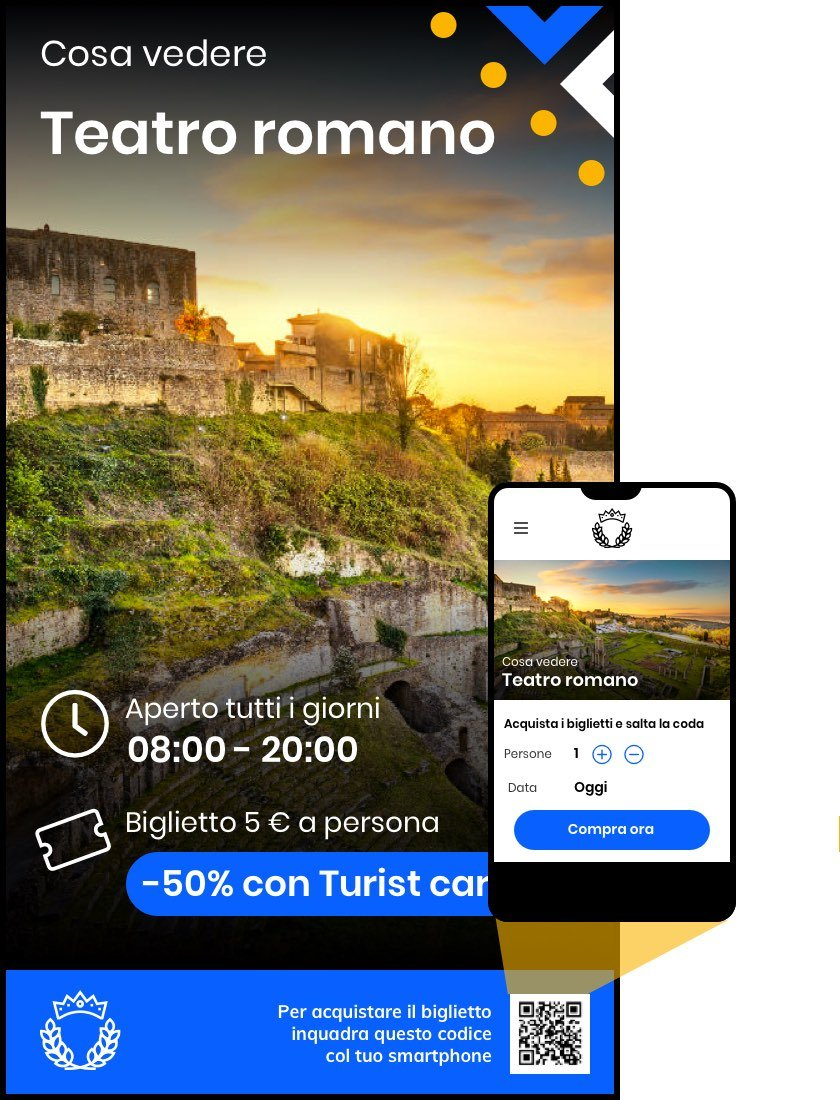
\includegraphics[width= 0.5\textwidth]{images/Introduzione/LiveTurist.jpg} 
    \caption{LiveSignage per scopi turistici.} 
\end{figure}

Inoltre, tramite un codice QR creato automaticamente insieme ai contenuti mostrati, l'utente finale può ricevere le informazioni in modo più dettagliato sul proprio dispositivo mobile senza bisogno di scaricare applicazioni o fare ricerche online.

\tomodify{I casi d'uso sono molteplici: cinema, ristoranti, turismo, sanità e soluzioni personalizzate, per fare alcuni esempi.
Tramite l'utilizzo di alcuni plugin è inoltre possibile ampliare ancora le possibilità del servizio come la possibilità di fare webcall e l'integrazione di social network.}

\section{Stato dell'arte}

All'inizio del tirocinio LiveSignage era già disponibile per dispositivi di Samsung e Raspberry.  

L'idea alla base dell'applicazione è quella di mostrare una serie di slide organizzate in playlist; ogni slide può mostrare diversi tipi di contenuti come ad esempio immagini, video, web page, mappe, social network, input esterni. Le playlist possono essere di diverso tipo:

\begin{itemize}
    \item Semplici: le slide vengono mostrate a schermo intero e si susseguono continuamente;
    \item Composte: in questo caso lo spazio a disposizione viene suddiviso in più parti e in ognuna di queste viene mostrata una playlist diversa;
    \item Concatenate: vengono concatenate più playlist una dopo l'altra.
\end{itemize}

\tomodify{Oltre alle semplici playlist è possibile anche inserire dei plugin per poter dare al cliente più possibilità di personalizzazione }, questi ad esempio permettono di  mostrare contenuti interattivi utilizzando l'input dell'utente tramite il touchscreen o di inserire il proprio e-commerce.

\subsection{Architettura}
\begin{figure}[!htb]
    \centering
    \includegraphics[width= 0.8\textwidth]{images/Introduzione/architettura.jpg} 
    \caption{Architettura dell'applicazione.} 
    \label{fig:architettura}
\end{figure}

\tomodify{immagine dell'architettura da modificare: \url{https://miro.com/app/board/uXjVOjz-X_4=/}}

\tomodify{L'applicazione è installata direttamente sul device, il cliente può impostare le playlist o eventuali modifiche del sistema come: timer di accensione e spegnimento, fuso orario, volume e luminosità, direttamente da un browser o dall'applicazione per dispositivi mobili (Figura: \ref*{fig:schermata-web}).\nl
Queste modifiche vengono inviate, tramite chiamate API al BackOffice che attraverso una socket si occupa di comunicare all'applicazione i cambiamenti avvenuti. 
L'applicazione utilizza le API del device per settare le modifiche di sistema e scrivere i file necessari per il mantenimento dei database e il salvataggio degli assets necessari: immagini e video. \n
Sono utilizzati due database: il primo è usato per salvare tutte le informazioni sulle playlist inserite fino a quel momento, eventuali timer, ID del dispositivo e altre informazioni utili al corretto funzionamento, il secondo salva i messaggi, tipicamente di errore, dell'applicazione; questo serve per permettere al cliente di scaricare questi messaggi in caso di problemi.\n
Le immagini e i video scaricati vengono salvati sul dispositivo e non saranno cancellate a meno di una richiesta specifica del cliente o in caso di necessità di liberare memoria. Questo per evitare di scaricare più volte lo stesso file.}\n

La figura \ref*{fig:architettura} mostra in maniera schematica l'architettura dell'applicazione e l'interazione con l'utente finale.

\begin{figure}[!htb]
    \centering
    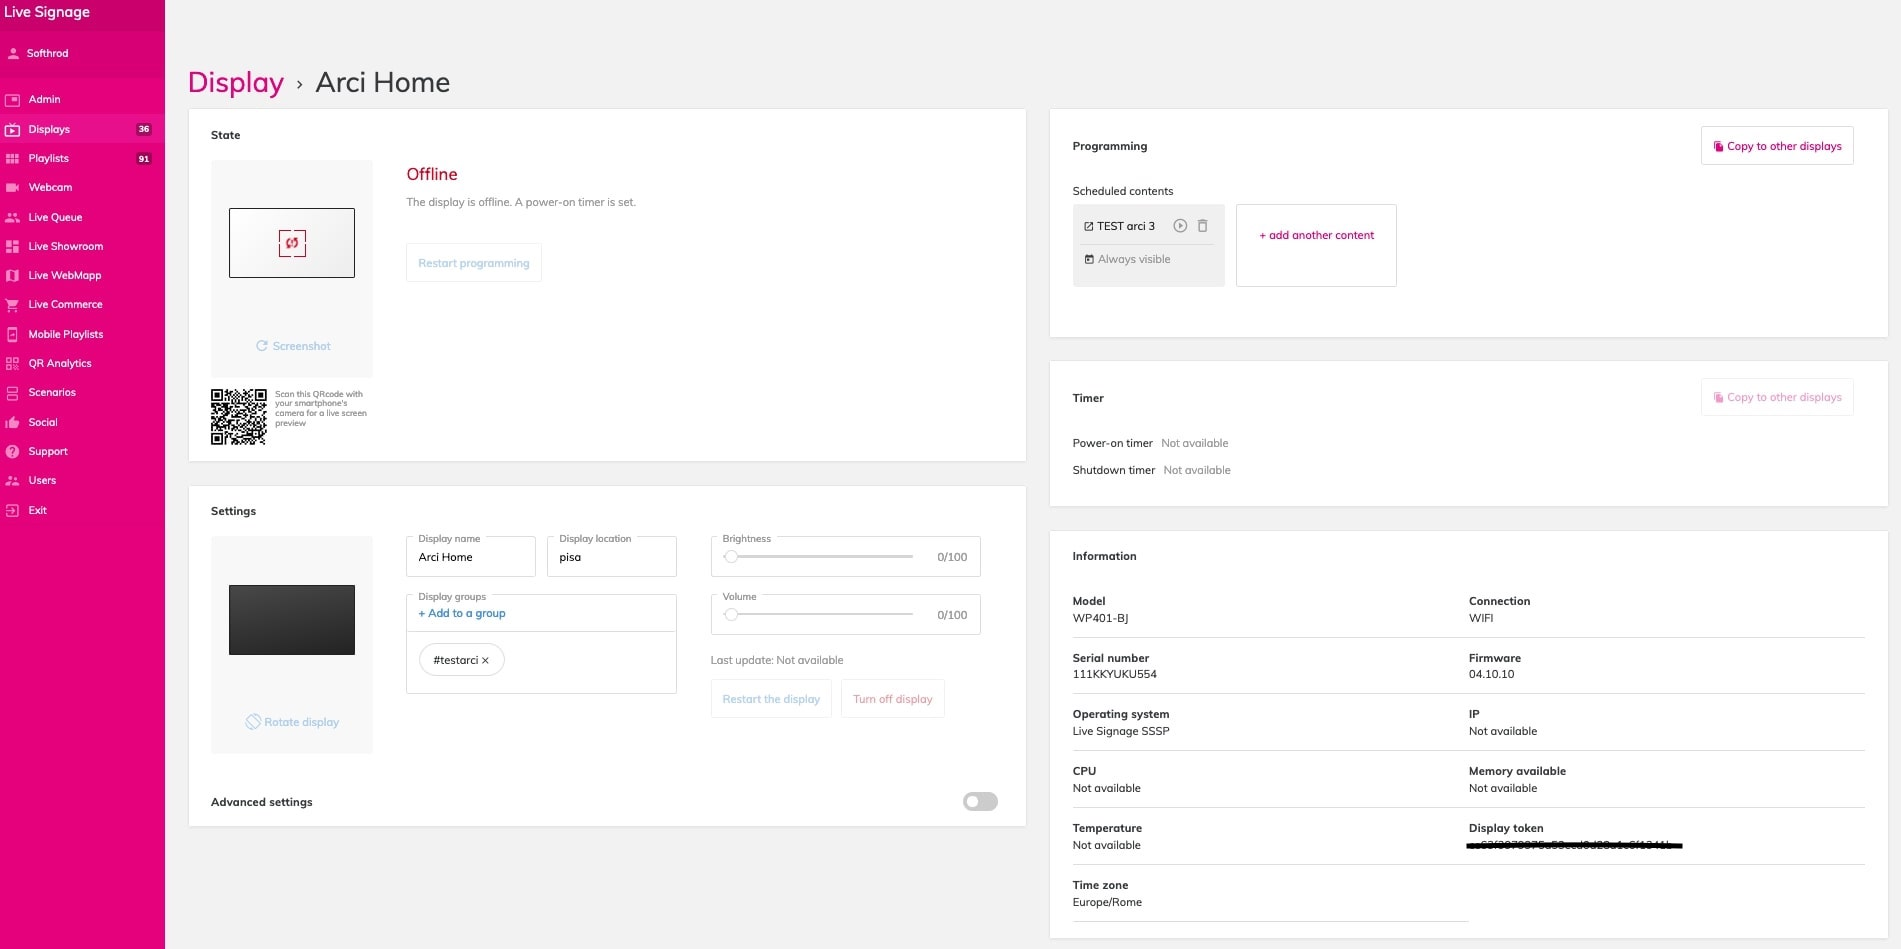
\includegraphics[width= 1\textwidth]{images/Introduzione/SchermataWebLS.jpg} 
    \caption{Schermata della Web Page per programmare il display.} 
    \label{fig:schermata-web}
\end{figure}

\section{Obiettivi raggiunti}

Al termine del tirocinio la versione di LiveSignage per WebOS Signage è stata correttamente sviluppata; ho avuto inoltre modo di aggiungere, o almeno studiare la possibilità di farlo alcune funzionalità non presenti nella versione per dispositivi Samsung, le quali non erano previste a inizio tirocinio, che lo studio della documentazione ci ha portato a considerare.

\section{Struttura della Relazione}
Di seguito una breve descrizione della suddivisione in capitoli di questa relazione.
\begin{itemize}
    \item Tecnologie utilizzate: Descrizione delle tecnologie a disposizione, loro differenze e scelte implementative da queste derivanti. Linguaggi e librerie utilizzate.
    \item LiveSignage su WebOs: Descrizione del lavoro svolto, difficoltà incontrate e soluzioni trovate, modifiche all'applicazione pre-esistente. Descrizione della fase di testing finale.
    \item Studio di funzionalità aggiuntive: In questo capitolo si presenta una descrizione della fase di analisi e, quando possibile, aggiunta delle nuove funzionalità e alcune idee per possibili miglioramenti futuri.
    \item Conclusioni: Riassunto dei punti principali affrontati e degli obiettivi raggiunti. Competenze acquisite.
\end{itemize}